\documentclass[aps,prl,superscriptaddress]{revtex4-2}

\usepackage{rotating} 
\usepackage{times}
\usepackage{graphicx}
\usepackage{setspace}
\usepackage{amsmath}
\usepackage{epstopdf}
\usepackage[obeyFinal]{easy-todo}
\usepackage{booktabs}
\usepackage{xr}

\makeatletter
\newcommand*{\addFileDependency}[1]{% argument=file name and extension
  \typeout{(#1)}
  \@addtofilelist{#1}
  \IfFileExists{#1}{}{\typeout{No file #1.}}
}
\makeatother

\newcommand*{\myexternaldocument}[1]{%
    \externaldocument{#1}%
    \addFileDependency{#1.tex}%
    \addFileDependency{#1.aux}%
}

\externaldocument{MANUSCRIPT/manuscriptSUPPL}

\begin{document}

\title{NMRlipids III: Lipid--Cholesterol Interactions in Atomistic Molecular Dynamics Simulations}

\author{Fernando Favela-Rosales}
\affiliation{Departamento de F\'isica, Centro de Investigaci\'on y de Estudios Avanzados del IPN, Apartado Postal 14-740, 07000 M\'exico D.F., M\'exico}
%
\author{Peter Heftberger}
\affiliation{Institute of Molecular Biosciences, Biophysics Division, NAWI Graz, University of Graz, Graz 8010, Austria}
%
\author{Matti Javanainen}
\email{matti.javanainen@helsinki.fi}
\affiliation{Institute of Organic Chemistry and Biochemistry,
Academy of Sciences of the Czech Republic, 
Prague 6, Czech Republic}
\affiliation{Institute of Biotechnology, University of Helsinki}
%
\author{Jesper J. Madsen}
\affiliation{Department of Global Health, College of Public Health}
\affiliation{University of South Florida}
%
\author{Josef Melcr}
\affiliation{Institute of Organic Chemistry and Biochemistry,
Academy of Sciences of the Czech Republic, 
Prague 6, Czech Republic}
%
\author{Markus Miettinen}
\affiliation{MPI}
%
\author{O. H. Samuli Ollila}
\email[]{samuli.ollila@helsinki.fi}
\affiliation{Institute of Organic Chemistry and Biochemistry,
Academy of Sciences of the Czech Republic, 
Prague 6, Czech Republic}
\affiliation{Institute of Biotechnology, University of Helsinki}
%
\author{Georg Pabst}
\affiliation{Institute of Molecular Biosciences, Biophysics Division, NAWI Graz, University of Graz, Graz 8010, Austria}
\affiliation{BioTechMed-Graz, Graz 8010, Austria}
%
\author{Thomas Piggot}
\affiliation{School of Chemistry, University of Southamptaon, Southampton SO17 1BJ, United Kingdom}
\affiliation{Chemical Biological and Radiological Sciences, Defence Science and Technology Laboratory, Porton Down, Salisbury, Wiltshire SP4 0JQ, United Kingdom}

\todo{Update Author list \& Affiliations}

\date{\today}

\begin{abstract}
Cholesterol is a central building block in biomembranes, where it induces orientational order, slows down diffusion, and thereby renders the membrane stiffer. Molecular dynamics simulations have played a crucial role in resolving these effects and the underlying molecular picture, yet it has recently become evident that different simulation models predict quantitatively different behavior. Such limitations are easily neglected, as the field rapidly progresses towards simulations of complex membranes mimicking the \textit{in vivo} conditions. Still, for their validity, it is crucial that the interactions between the fundamental building blocks of biomembranes, such as phospholipids and cholesterol, are modelled accurately.
%
Here, we perform a systematic comparison of the ability of commonly used force fields to describe the structure and dynamics of binary mixtures of phosphatidylcholine and cholesterol. Comparison of lipid bilayer simulations with deuterium order parameters and lateral diffusion coefficients from NMR as well as form factors from X-ray scattering reveals that none of the existing force field outperforms the others across the physiologically relevant cholesterol concentrations. The Amber-compatible force fields show the smallest deviations from experiment with Slipids and Lipid17 models excelling at low and high cholesterol concentrations, respectively. 
%The performance of the commonly used CHARMM36 model is subpar, as it overestimates diffusion at low cholesterol concentrations, and gets excessively ordered upon the addition of cholesterol. 
The accompanied X-ray scattering data set measured for this work will foster future force field development and refinement.
\end{abstract}

\maketitle

\section{Introduction}

\todo{Check that the uses of ``model'' and ``force field'' are consistent}

Cellular membranes contain an incredibly complex mixture of lipid molecules \cite{lorent2020plasma} which are unevenly distributed in the membrane plane and across its leaflets \cite{van2008membrane,wang2020membrane,kinnun2020lateral}. A key player driving the lateral heterogeneity is cholesterol (CHOL), which is present at concentrations between $\sim$10~mol-\% (endoplasmic reticulum) and up to $\sim$50~mol-\% (plasma membrane) \cite{van2008membrane}. CHOL has the unique ability to order neighbouring lipids and thus induce the liquid ordered (L\textsubscript{o}) phase in model membranes \cite{mouritsen2004s,ipsen87,kinnunen91,rog2009ordering}. In the cellular setting, the interaction between phospholipids and CHOL is associated with the formation of lipid rafts and nanodomains \cite{Simons97,cebecauer2018membrane}. This heterogeneity can then further regulate protein distribution \cite{milovanovic2015hydrophobic} or conformation \cite{kelkar2007modulation} \textit{via} the hydrophobic mismatch mechanism \cite{killian1998hydrophobic}, in addition to the direct modulation of protein function \cite{gimpl2016interaction,guixa2017membrane}.

While detailed experimental information of the interactions among phospholipids and CHOL is relatively sparse, atomistic resolution molecular dynamics (MD) simulations have been widely applied to provide a detailed view of the lateral organization of lipid bilayers as well as lipid--CHOL interactions \cite{rog14,rog2009ordering,berkowitz2009detailed}. However, the trustworthiness of any prediction from an MD simulation relies on the quality of the used model. Fortunately, in addition to constant refinement of existing parameters, atomistic \emph{force fields} have also seen the expansion to other classes of biomolecules, including lipids, sugars, and nucleic acids \cite{leonard2019developing,marrink2019computational}. The traditional protein force fields CHARMM \cite{brooks1983charmm}, AMBER \cite{cornell1995second}, and OPLS \cite{jorgensen1988opls,harder2016opls3} now have growing libraries of compatible lipid molecules, including CHOL, in the forms of CHARMM36 \cite{Klauda06,lim12}, Lipid17/Slipids \cite{dickson14,madej15,jambeck12,jambeck12b,jambeck13b,grote2020optimization}, and the model by Maciejewski and Rog (here ``MacRog'') \cite{maciejewski14,kulig14,kulig15,Kulig15b}, respectively. Moreover, OPLS3e \cite{harder2016opls3} contains parameters for lipids, but CHOL is currently not included. 

Thanks to the compatibility with protein force fields, the lipid models can be used in studies of membrane proteins or protein--membrane interactions in addition to sole lipid membranes. Notably, simulations using CHARMM36, Lipid17, and Slipids are now readily set up using CHARMM-GUI for multiple simulation engines \cite{lee16,lee2020charmm}. Despite this ease-of-use, the choice of a force field for an MD simulation can be challenging, as each model comes with its own set of pros and cons. Unfortunately, careful comparisons of force field quality, especially for capturing the features of lipid mixtures, are scarce in the literature. This largely results from the lack of availability of systematic, comprehensive, and quantitative datasets from both experiments and simulations.

We have previously performed such comparisons for the structure of phosphatidylcholine (PC) lipids \cite{botan15}, for PC--ion interactions \cite{catte2016molecular}, for phosphatidylserine (PS) lipids \cite{antila2019headgroup}, and for phoshatidylethanolamine (PE) and phosphatidylglycerol (PG) lipids \cite{bacle2021inverse}. Here, we extend this work to mixtures of PC and CHOL. We compare the ability of popular force fields to reproduce effects of CHOL on the structure and dynamics of a PC lipid bilayer, and thereby set guidelines for future efforts to validate intermolecular interactions in binary and more complex systems. Moreover, if some of the studied force fields satisfactorily reproduce experimental behavior at least in some range of CHOL concentrations, the molecular level picture provided by it can be assumed to mimic reality in this concentration regime. 

Our earlier work has demonstrated that the structural ensembles of lipids from an MD simulation can be directly compared to those from solid state NMR experiments \cite{botan15,catte2016molecular,antila2019headgroup,bacle2021inverse}. This approach based on order parameters is quantitative, has small error estimates, is highly reproducible, and does not suffer from perturbation of probes used in many other techniques. Thus, we compare our simulation results with different force fields to the systematic NMR data set of PC C--H bond order parameters with varying CHOL concentrations \cite{ferreira13}. In addition, we measured form factors for a range of PC--CHOL mixtures using small angle X-ray scattering, and used them to subsequently model the electron density profiles across the lipid bilayer. The form factor and electron density profiles can be compared with the same profiles calculated from the simulation data. Whereas NMR provides data on the conformations of individual lipids, form factors from scattering captures the details of the structure of the entire lipid bilayer \cite{ollila16}. 

One limitation in comparing simulations of lipid mixtures with experimental data is that the various experiments are performed at different concentrations, and thus mimicking all compositions in simulations is tedious. Here, we demonstrate that if the simulations and experiments sample multiple CHOL concentrations, the order parameters and electron density profiles can be readily interpolated to intermediate CHOL concentrations. This enables the comparison of data sets that are not extracted at the exact same CHOL concentrations, as is usually the case, especially if multiple techniques are combined in the comparison. 

We also evaluated whether the simulation force fields reproduce the dependence of lateral diffusion coefficients on cholesterol measured using pulsed field gradient (PFG) NMR \cite{filippov2003effect,filippov2003influence}. This comparison is enabled by the recent theoretical work that allows for the elimination of finite-size effects in MD simulations and thus a quantitative comparison with experiment \cite{vogele2016divergent,vogele2018hydrodynamics}. With the structural and dynamic comparisons established, we estimated the quality of each force field at different CHOL concentrations. We then analyzed the molecular organization in the best-performing force field at low and high CHOL range, as we expect them to best reflect this organization in reality.

\section{Methods}

\subsection{X-ray Scattering Experiments}

\todo{Complete scattering methods}

%Such scattering experiments are challenging to interpret for multi-component lipid bilayers \cite{pan12,Heftberger15,Marquardt15}, yet we still extract  thus area per molecule values, one of the main quantity used to compare simulations to experiments, have not been available for lipid cholesterol mixtures. 

We measured small angle X-ray scattering (SAXS) data on multilamellar vesicles (MLVs) composed of POPC and CHOL with the latter present at 0--50~mol-\% with 5~mol-\% increments. The data were obtained at the EMBL BioSAXS beamline (Hamburg) using 20~keV photons at $T=300$~K and analyzed in terms of the SDP-GAP model described in Refs.~\citenum{Heftberger.2014} and \citenum{Heftberger15}. The data from MLVs contain the structure factor (the crystalline lattice) and form factor in a convoluted fashion, yet by fitting the scattered intensity data we obtain both contributions. In this work, only the form factors are discussed. The electron density profiles have been modelled in terms of the SDP model \cite{heberle12,Kucerka08a,kucerka12}, \textit{i.e.} volume distribution functions are modelled by individual Gaussians or error functions. CHOL is particularly challenging to describe within the SDP model, and therefore form factors are often compared between simulation and experiment \cite{Kucerka08b} instead of density profiles, or CHOL density is modeled together with that of CH$_2$ groups \cite{pan12}. Here, cholesterol is accounted for by two Gaussians, as proposed by Jianjun Pan (private communication), and used in Refs.~\citenum{belivcka2017high} and \citenum{heftbergerthesis}. 
%Additional figures show the volume distribution functions and the resulting electron density profiles.
%Authors to consult and potentially include in publications using this data: Peter Heftberger (peter.heftberger@gmx.at), Georg Pabst (georg.pabst@uni-graz.at)

\subsection{Molecular Dynamics Simulations}

We performed MD simulations of a pure POPC membrane as well as five POPC/CHOL mixtures with CHOL content ranging from 11 to 47~mol-\%. In order to eliminate the finite size effects due to periodic boundary conditions from lateral diffusion coefficients of lipids, we performed all simulations in three sizes. The small (64 POPC molecules) and medium (256 POPC molecules) systems were only used in the diffusion analysis, whereas all other analyses were performed on the large membranes (1024 POPC molecules). The number of POPC molecules was kept constant across the different CHOL concentrations. All membranes were solvated by 50 waters per lipid (POPC or CHOL). The simulations were performed using four commonly used force fields, namely CHARMM36 \cite{Klauda06,lim12}, Amber-compatible Slipids \cite{jambeck12,jambeck12b,jambeck13b} with its 2020 update \cite{grote2020optimization}, Amber-compatible Lipid17 \cite{dickson14,madej15}, and OPLS-aa-compatible MacRog \cite{kulig14,kulig15,Kulig15b} models. All simulations were 1~\textmu{}s long, totaling 72~\textmu{}s, and performed using GROMACS version 2020 or 2021 \cite{pall2020heterogeneous}. The used simulation parameters are provided in Table~\ref{SItab:params}, and the simulation data are available at DOI: 10.5281/zenodo.7035350 (CHARMM36), DOI: 10.5281/zenodo.7022749 (Slipids), DOI: 10.5281/zenodo.6992065 (Lipid17), and DOI: 10.5281/zenodo.7061800 (MacRog).

\todo{Run Lipid21 for revision?}

\begin{table*}[]
\begin{center}
    \caption{\label{tab:simulations}%
    Details of the simulation systems provided for (small/medium/large) system sizes). The box dimensions in the membrane plane ($x/y$) and normal to the membrane ($z$) are provided for the Slipids simulations, and the values vary slightly between the force fields.
    }
    \begin{tabular}{c|ccccc}
    \toprule
    $[$CHOL$]$ & POPC & CHOL & Water & $x/y$ (nm) & $z$ (nm) \\
    \midrule
    0~mol-\%    & 64/256/1024 & 0/0/0       &   3200/12800/51200 & 4.4/9.0/18.1 & 8.9/8.6/8.5    \\
    11~mol-\%   & 64/256/1024 & 8/32/128    &   3600/14400/57600 & 4.5/9.4/18.1 & 9.4/9.1/9.3    \\
    20~mol-\%   & 64/256/1024 & 16/64/256   &   4000/16000/64000 & 4.5/9.2/18.3 & 10.2/9.9/10.0  \\
    29~mol-\%   & 64/256/1024 & 26/104/416  &   4500/18000/72000 & 4.6/9.2/18.5 & 10.8/10.8/10.7 \\
    38~mol-\%   & 64/256/1024 & 40/160/640  &   5200/20800/83200 & 4.8/9.5/19.2 & 11.3/11.4/11.2 \\
    47~mol-\%   & 64/256/1024 & 56/224/896  &   6000/24000/96000 & 5.0/10.1/20.0 & 11.8/11.6/11.7 \\
    \bottomrule
    \end{tabular}
\end{center}
\end{table*}

\subsection{Simulation Analyses}

\paragraph{Electron Density Profiles and Bilayer Dimensions:} The form factors and electron density profiles were calculated using the \texttt{form\_factor.py} script in the NMRlipids Databank (\url{https://github.com/NMRLipids/Databank/}) after assigning all atom types with valence electron counts. The thicknesses were extracted by the \texttt{findpeaks} function in Matlab after smoothening the electron density data. Area per phospholipid was obtained by dividing the area of the bilayer by the number of phospholipids in one leaflet. 

\paragraph{Order Parameters:} The C--H order parameters were calculated as
%
\begin{align}
    S_\mathrm{CD}=\left\langle\frac{3\cos^2\theta-1}{2}\right\rangle,
\end{align}
%
where $\theta$ is the angle between the C--H vector and the $z$ axis normal to the bilayer plane. In the POPC acyl chains, the values for the 2 (3) hydrogens of CH$_2$ (CH$_3$) groups were averaged, since these groups rotate freely and thus the order parameters are identical for both (all) hydrogens in experiments. In simulations, the values are also very similar, justifying this approach. An exception to this are the hydrogens bound to the 2\textsuperscript{nd} carbon in the oleate chain; they lack rotational averaging in both both simulations and experiments, and were thus treated separately in our analyses. The C--H order parameters for the POPC head group were calculated similarly, but values for both hydrogens are shown separately for all CH$_2$ groups, \textit{i.e.} no averaging was performed. 

\paragraph{Lateral Diffusion Coefficients:} The lateral diffusion coefficients $D_\mathrm{PBC}$ from simulations performed using periodic boundary conditions (PBC) were extracted from mean squared displacement (MSD) data calculated for lipid centers of mass after eliminating the drift of their host leaflet with the \texttt{gmx msd} tool. The MSD data were fit with a straight line in the lag time ($\Delta$) interval between 10 and 100~ns as
%
\begin{align}
	\mathrm{MSD}=4D_\mathrm{PBC}\Delta.
\end{align}

The diffusion coefficients extracted from the three simulation box sizes were fitted with
%
\begin{align}
	D_\mathrm{PBC}\approx D_\infty+\frac{k_\mathrm{B}T}{4\pi\mu_\mathrm{m}h}\frac{\ln\left[L/\left(L_\mathrm{SD}+1.565H\right)\right]-1.713}{1+H/L_\mathrm{SD}},
	\label{eq:sdlatpbc}
\end{align}
%
where $D_\infty$ is the lateral diffusion coefficient in an infinite system, $h$ is the hydrodynamic thickness of the membrane, $k_\mathrm{B}T$ is the Boltzmann constant, $T$ is the temperature, $mu_\mathrm{m}$ and $mu_\mathrm{f}$ are shear viscosities of the membrane and the fluid (water), respectively. $H$ is half the thickness of the water layer and $L_\mathrm{SD}=\frac{h\mu_\mathrm{m}}{2\mu_\mathrm{f}}$ the Saffmann--Delbr\"{u}ck length \cite{vogele2018hydrodynamics}. The inter-leaflet friction coefficient does not appear in Eq.~\eqref{eq:sdlatpbc} as we expect it to be infinite, which was found to be a valid assumption for lipid bilayers \cite{vogele2018hydrodynamics}. The water viscosity value of 0.3228~mPa$\cdot$s was interpolated to 298~K from the values for CHARMM TIP3P in Ref.~\citenum{ong2019temperature} and used for all simulations (CHARMM TIP3P and normal TIP3P differ by $\sim$2--3\%). The final simulation box dimensions were used for $L$ and $H$. For $h$ and $H$ ($=(L_z-h)/2$, the average values from the three systems sizes were used. 

\paragraph{More and Less Ordered Populations:} The angles ($\theta$) between the C--H vectors of the last six carbons of the palmitate chain were extracted and the data across all CHOL concentrations was accumulated. These data were fit with two Gaussians centered at 0,
%
\begin{align}
    P(\theta)=a_\mathrm{less}\exp\left(-\frac{\theta}{2\sigma_\mathrm{less}}\right)+a_\mathrm{more}\exp\left(-\frac{\theta}{2\sigma_\mathrm{more}}\right),
    \label{eq:twogauss}
\end{align}
%
where the two standard deviations ($\sigma$) correspond to the more and less ordered components. After these $\sigma$ values were established for a given force field, the data at all CHOL concentrations was independently fitted by Eq.~\eqref{eq:twogauss} with fixed $\sigma$ values. These fits provided the pre-factors, whose ratio $a_\mathrm{more}/(a_\mathrm{more}+a_\mathrm{less})$ corresponds to the fraction of the more ordered component in the system. 

This two-Gaussian approach assumes a ``two-population'' scheme, where the more and less ordered populations are present (at non-zero CHOL concentration), and that the addition of CHOL only affects their ratio, but not the nature. In an alternative picture of a ``collective transition'', there would be a single Gaussian, whose standard deviation $\sigma$ would vary systematically as a function of CHOL concentration.

\paragraph{Quantitative Quality Measure for Lipid Bilayer Structure:} The deviations (in \%) from experimental values across CHOL concentrations were used to quantify the quality of the lipid force fields. The density profiles (as a function of distance from membrane core along the membrane normal), oleate and palmitate chain order parameters (as a function of carbon atoms in the acyl chains), and diffusion coefficients were interpolated to create continuous 2D matrix for density profiles and order parameters, and a continuous 1D vector for the diffusion coefficients. For the 2D matrices, the absolute values of the differences of the matrices from simulations and experiments were calculated and averaged over one dimension which was either the distance from membrane core or the carbon atom number, respectively. This resulted in a 1D deviation vector as a function of CHOL concentration. For diffusion coefficients, the absolute value of the difference of the interpolated 1D vectors of simulation and experimental data was calculated to provide deviation as a function of CHOL concentration. All these 1D vectors were normalized by dividing them by the experimental values to provide relative deviations in \%.

\section{Results and Discussion}

\todo{Results: volmaps of chains around cholesterol?}\\
\todo{Results: SI: RDFs of POPC/CHOL around CHOL}\\
\todo{FF minima analysis}

\subsection{Cholesterol Condensing Effect is Manifested Differently in Different Force Fields}

Lipid bilayer dimensions can be experimentally accessed by measuring X-ray scattering form factor, which is related to the electron density along membrane normal \textit{via} a Fourier transform \cite{pan12,Heftberger15,Marquardt15,ollila16,??}. The form factor can be translated to an electron density profile, and area per lipid and bilayer thickness values can be extracted using the scattering density profile (SDP) model or its combination with MD simulations  \cite{pan12,Heftberger15,Marquardt15,??,doktorova2020molecular}. Sophisticated approaches for single component lipid bilayers are available but the data for multi-component systems are more difficult to interpret, and the used approaches involve severe approximations \cite{pan12,Heftberger15,Marquardt15,??}. 

Thus, we compare here the total electron density profiles which do not require the de-convolution of the electron density profiles into densities of the different molecular species. For reference, all form factor profiles from experiment and simulation are shown in Fig.~\ref{SIfig:scattering}. As the absolute and relative lobe amplitudes depend on simulation box size (Fig.~\ref{SIfig:scatteringvssize}), the minima in the form factor profiles provide a robust comparison between simulation and experiment. Thus, we have also traced the minima in these profiles, and they are plotted in Fig.~\ref{SIfig:ffminima}. As simulations and experiments were performed at somewhat different CHOL concentrations, we generated two-dimensional maps for the density profiles using interpolation (see Methods). These maps are shown in Fig.~\ref{fig:densmaps} for both simulations (top row) and experiment (bottom row, left column). The original electron density profiles used in the generation of these maps are shown in Fig.~\ref{SIfig:densprofs}.

\begin{figure}[htb!]
  \centering
  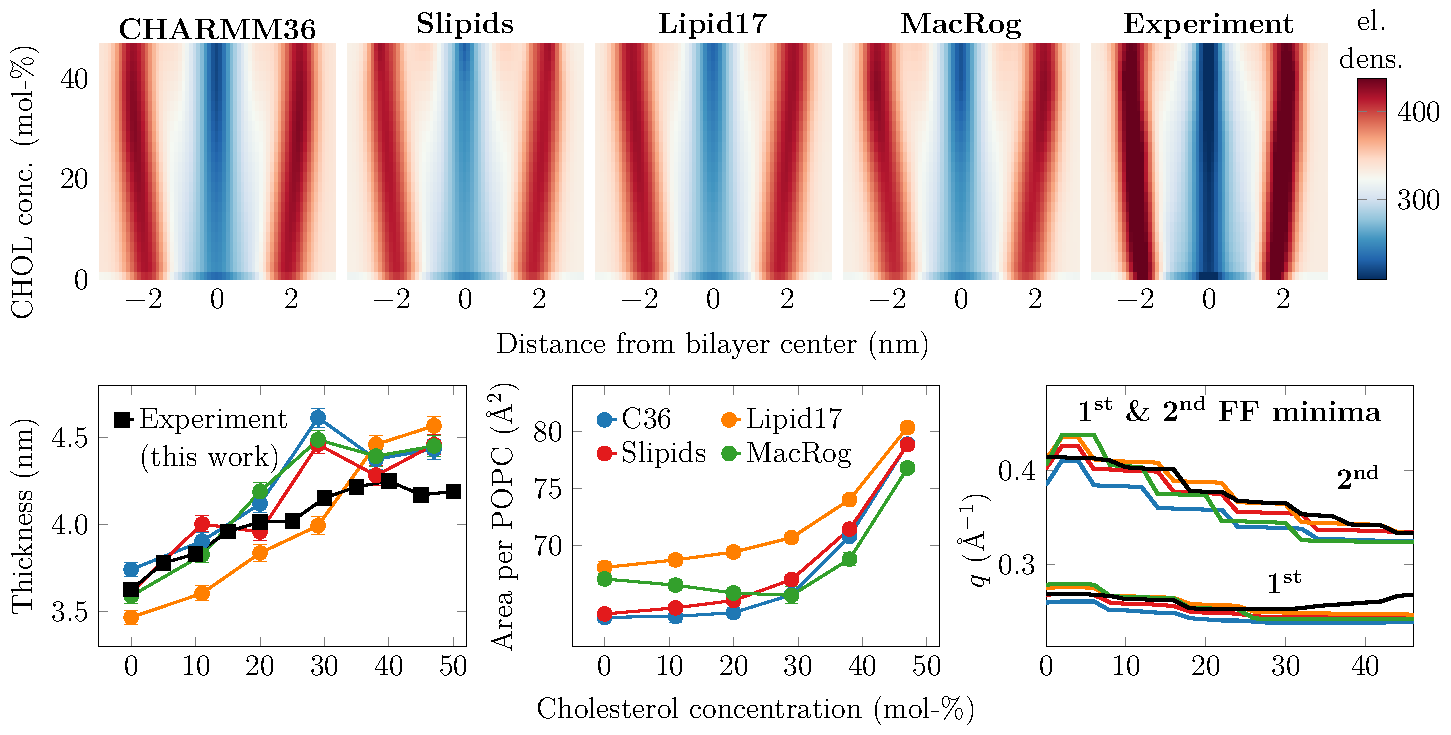
\includegraphics[width=\linewidth]{../FIGS/densitymaps.pdf}
  \caption{\label{fig:densmaps}%
  \textbf{Electron density profiles, thickness and area per lipid as a function of CHOL concentration.}
  %
  Top: Electron density maps for the simulations using four different force fields.
  %
  Bottom left: Electron density map for the experiment. The scaling is uniform between all simulations and experiment. The original electron density profiles are shown in Fig.~\ref{SIfig:densprofs}. The scattering experiments are interpolated to 298~K from Refs.~\citenum{pabst2000structural} (58.8~\AA{}$^2$), \citenum{kuvcerka2006structure} (67.5~\AA{}$^2$), and \citenum{Kucerka11} (63.5~\AA{}$^2$). The NMR data is measured in Ref.~\citenum{Leftin14} using either $^{13}$C (58.9~\AA{}$^2$) or $^2$H (58.3~\AA{}$^2$) NMR. The effect of system size on the density profiles in simulations is demonstrated in Fig.~\ref{SIfig:densprofssize} in the SI.
  %
  Bottom center: Bilayer thickness. Thickness is defined as twice the distance from the peak in electron density to the membrane core. Experimental data are extracted in a similar manner from electron density profiles obtained with X-ray scattering.
  %
  Bottom right: area per lipid measured by dividing the total membrane area by the number of phospholipids. 
  %
  The size-dependency of area per lipid is shown in Fig.~\ref{SIfig:aplvssize}.
  }
\end{figure}

Overall, all electron density profiles share the same features across all CHOL concentrations; a high-density band corresponding to the tightly-packed interfacial region rich in electron-rich phoshorus, a low-density region at the core of the membrane occupied by the disordered acyl chains, and intermediate density in the rest of the lipid regions as well as the aqueous phase. However, a more detailed look at the profiles in Fig.~\ref{fig:densmaps} reveals differences between the force fields. CHOL renders the membrane thicker, resulting in the deviation of the high-density bands with increasing amount of CHOL. In CHARMM36, Slipids, and MacRog, there is clear saturation of this effect at around 30~mol-\% CHOL. In Lipid17, however, the membrane gets thicker until the maximum studied CHOL concentration of 47~mol-\%. In experiment, the effect of CHOL is generally weaker, and some saturation is evident at high CHOL concentrations. These trends are visible in the bottom middle panel in Fig.~\ref{fig:densmaps}, which shows the effect of CHOL on membrane thickness. Fig.~\ref{fig:densmaps} also demonstrates that CHARMM36 has the sharpest low- and high-density bands indicating, and the same is true for MacRog at higher cholesterol concentrations. This uniform membrane structures could indicate small undulations, whereas the less sharp Lipid17 and especially Slipids profiles could indicate a more flexible membrane. 

Comparison against experiments (bottom left panel in Fig.~\ref{fig:densmaps}) indicates that the membrane structure is more uniform in the experiment, as the bands are sharper. This is also evident in the original electron density profiles in Fig.~\ref{SIfig:densprofs}. System size plays a role here, as demonstrated by the density maps calculated for the CHARMM36 simulations in three sizes, shown in Fig.~\ref{SIfig:densprofssize}. The larger the system, the larger the bilayer undulations are, which can smear the features of the density profiles. Still, even in the smallest system, the band intensities are not as localized as in the experiment.

Comparison of the thickness values (bottom middle panel in Fig.~\ref{fig:densmaps}) demonstrates that the Lipid17 bilayers are too thin at low CHOL concentrations, whereas other models agree well with experiment in this regime. Still, all simulation models overshoot the experiment at high CHOL concentrations. Experiment and all simulation models except Lipid17 demonstrate saturation after 30~mol-\%.

The membrane-condensing effect of CHOL is well documented, yet there is some ambiguity surrounding the term \cite{edholm2005areas}. The cross-sectional area of a CHOL molecule is smaller than that of a phospholipid, so an increase in CHOL concentration is expected to lower the average \emph{area per lipid} (including CHOL). However, condensation could also refer to a decrease in the \emph{area per phospholipid} upon the addition of cholesterol \cite{edholm2005areas}, or to CHOL having a diminishing partial area, \textit{i.e.} a certain amount of CHOL could be added to a phospholipid bilayer without increasing or decreasing its total area \cite{javanainen2017two}. We thus compared the behavior of the area per (POPC) lipid (APL) as a function of CHOL concentration in the bottom right panel of Fig.~\ref{fig:densmaps}. The dependence of APL on CHOL concentration follows the trends in thickness inversely in general, yet provide curious differences between the force fields. Lipid17 has the largest APL across the entire CHOL contration range, and the addition of CHOL always leads to an increase in the membrane area. MacRog also has a large APL for pure POPC, but the partial area of CHOL is negative until 30~mol-\% concentration indicating a particularly strong condensation effect. The profiles for Slipids and CHARMM36 are very similar, and the partial area of CHOL is small or even zero until a concentration of 20~mol-\%. Importantly, the observed differences in CHOL condensing effect take place at the physiologically relevant CHOL concentration range \cite{van2008membrane}. Experimental data are derived from models, so they can vary greatly, as evidenced by the very different values obtained by \citeauthor{pabst2000structural}\cite{pabst2000structural} and \citeauthor{kuvcerka2006structure}\cite{kuvcerka2006structure} for POPC at 303~K. 

\subsection{Acyl Chain Ordering Varies Greatly Between the Force Fields}

Order parameters for C--H bond vectors measured with with $^{13}$C or $^{2}$H NMR techniques, provide indirect information about the structural sampling of indidual molecules \cite{ollila16}. Moreover, these parameters are readily extracted from the simulation. An increase in acyl chain order parameters with added cholesterol in simulations and experiments can be explained by increased anti conformations in acyl chains \cite{ferreira13,??}, which is suggested to play critical role in the phase behaviour of PC--cholesterol mixtures \cite{ipsen87}. Consequently, the correct cholesterol ordering effect is expected to be a necessary condition for a model used to understand lipid--cholesterol phase behaviour.

Here, as the NMR experiment \cite{ferreira13} was again performed at different CHOL concentrations than simulations (and X-ray scattering measurements), we generated order parameter maps as a function of acyl chain carbon number and cholesterol concentration for both simulations and experiments, and subtracted these maps to obtain the deviation of simulation from experiment. These maps are shown for the palmitate (top row) and oleate (bottom row) chains of POPC in Fig.~\ref{fig:OPmaps}, whereas the original order parameter profiles are shown in Figs.~\ref{SIfig:palmitate} and \ref{fig:SIfig:oleate}.

\begin{figure}[htb!]
  \centering
  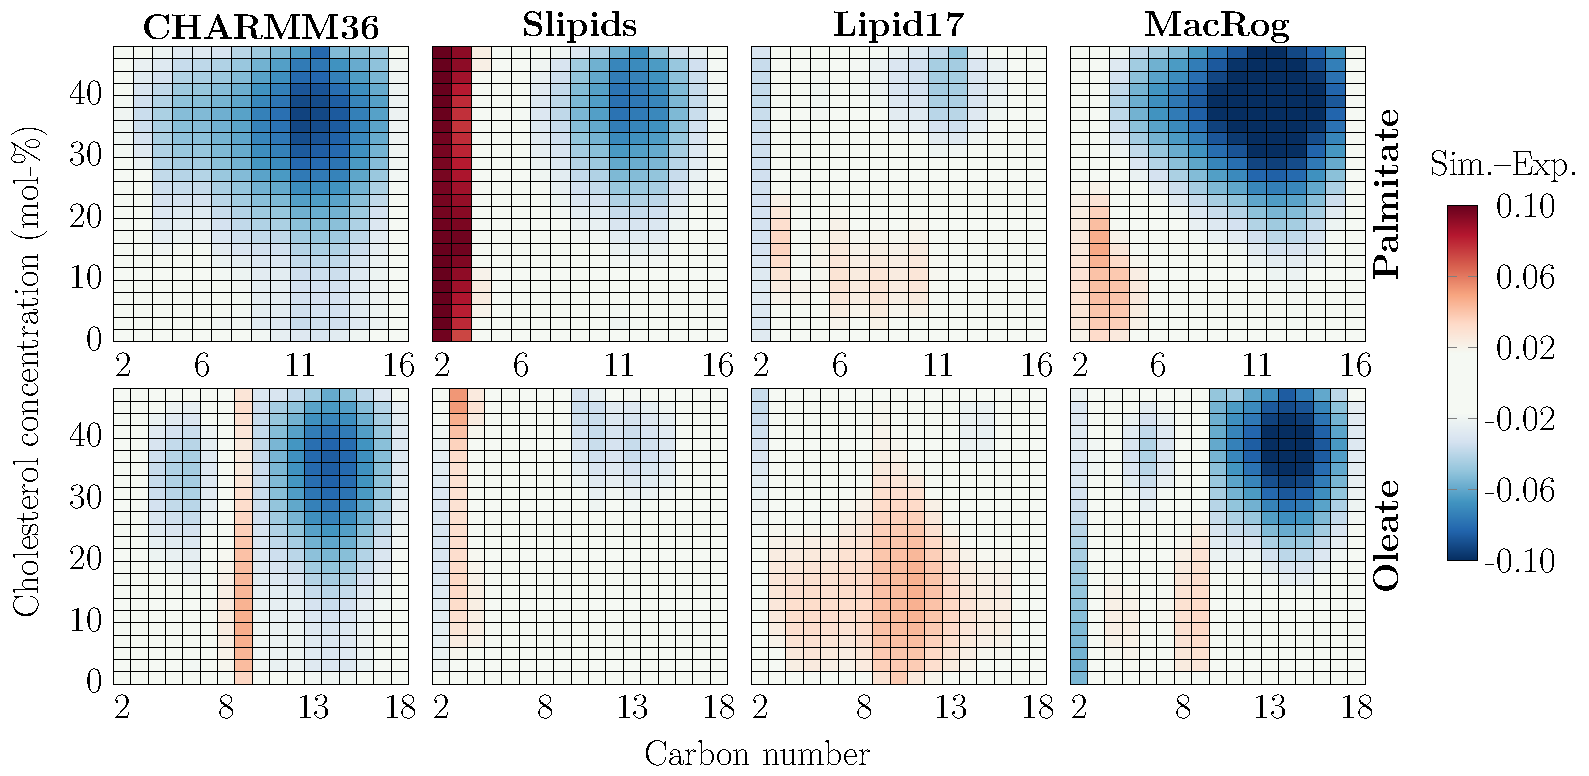
\includegraphics[width=\linewidth]{../FIGS/OP_chains.pdf}
  \caption{\label{fig:OPmaps}%
  POPC acyl chain order parameter deviation from experiments. Data are shown for palmitate (top row) and oleate (bottom row) and for our force fields (columns). Negative values indicate that order is too high ($-S_\mathrm{CD}$ values too negative) in the simulations. The values that are within the estimated error range of 0.02 from experiment are considered to be correct ``correct'' and coloured in white. The order parameters calculated for the two or three identical carbons were very similar and thus averaged over in simulations, as they have identical values in experiments. For the C2 carbon of the oleate chain, the order parameters are forked in simulations and experiments. We thus calculated the differences for both the larger and smaller values, and averaged this deviation for the C2 column of oleate.
  }
\end{figure}

These original maps in Fig.~\ref{SIfig:orderparameters} demonstrate that the addition of cholesterol substantially increases the acyl chain C--H order parameters for all simulation models and experiments, which can be explained by increased anti conformations in acyl chains \cite{ferreira13,??}. The absolute values of order parameters of \textit{sn}-1 chain from $^{13}$C NMR experiments \cite{ferreira13}
exhibit approximately linear increase with cholesterol up to equimolar mixture (Fig. \ref{slopes}), which is expected because
phase separation is not observed for this mixture \cite{ionova12,ferreira13}.

The deviations mapped in Fig.~\ref{fig:OPmaps} provide an intuitive way for a quantitative comparison of the behaviors of the force fields. Here, deviations in the range [$0.02$,0.02] are considered to fall within the error estimate and are thus shown in white. Blue indicates that the order parameters are too low in the simulation (their absolute value is larger, \textit{i.e.} the chains are too ordered). Overall, the simulation models behave reasonably well at low CHOL concentrations, but deviate significantly from experiment at higher CHOL concentrations. 

In CHARMM36, the both the palmitate and oleate chains get too ordered upon increasing CHOL concentration, yet the oleate C9 carbon next to the double bond is too disordered in the simulation. The oleate chain shows best agreement with experiment in Slipids with only slight excess ordering at higher CHOL concentrations. The excess ordering is more severe for the palmitate chain. Still, the major discrepancy between Slipids and experiment is the drastically too disordered C2 and C3 carbons of the palmitate chain. This effect was not present in the original Slipids model \cite{botan15}, indicating that it was introduced in the recent reparametrization that improved the head group and glycerol backbone structures of Slipids \cite{grote2020optimization}. Lipid17 provides the best overall agreement with experiment, as no segments deviate significantly from experiment at any CHOL concentrations. At low CHOL concentrations, the middle of the oleate chain is too disordered, which agrees with the large APL observed in Fig.~\ref{fig:densmaps}. At large CHOL concentrations, the oleate chain agrees well with experiment, whereas the palmitate chain has a slightly too ordered C9--C12 segment, yet the deviation is significantly smaller than in the other force fields. MacRog behaves reasonably well at low CHOL concentrations, yet the C2--C5 carbons in palmitate are slightly too disordered, whereas the C2 of oleate is somewhat too ordered. However, at larger CHOL concentrations the chains become overall way too ordered, leading to the largest overall deviations from experiment.

The head group order parameters are not largely affected by CHOL concentration in experiments \cite{ferreira13}, which has been discussed in our earlier work \cite{botan15}. The four force fields evaluated here also reproduce this behavior to a great degree (Fig.~\ref{SIfig:headgroups}), so the limitations observed in the absence of CHOL\cite{botan15} largely persist across all studied CHOL concentrations. Moreover, it has now become standard to consider them in the parameterization and validation of lipid force fields \cite{dickson2022lipid21,grote2020optimization,yu2021charmm36,yu2021semi}.

\todo{Also experimental cholesterol order parameters are available. Maybe these should be calculated from simulations as well.}

\subsection{The Force Fields Predict Very Different Lateral Mobilities}

Apart from the ordering effect on the bilayer structure, CHOL is also known to make them stiffer and less dynamic \cite{rog2009ordering,filippov2003effect,filippov2003influence}. The comparison between lateral diffusion coefficients extracted from simulation and experiment has been limited due to a box-size dependence observed in simulations performed using periodic boundary conditions \cite{vogele2016divergent,vogele2018hydrodynamics,camley2015strong}. Here, we tackle this issue by performing simulations with three system sizes, which allows the extrapolation of the results to an infinite system with the theoretical description developed by \citeauthor{vogele2016divergent}  \cite{vogele2018hydrodynamics,vogele2018hydrodynamics}. Importantly, reference values are available for POPC/CHOL mixtures from $^1$H pulsed field gradient NMR diffusion measurements on label-free macroscopically aligned bilayers. The PBC-corrected lateral diffusion coefficients are shown in the top panel of Fig.~\ref{fig:dynamics} together with experimental values. The size-dependence of these values extracted from simulations together with the fit of Eq.~\eqref{eq:sdlatpbc} are shown in Fig.~\ref{SIfig:dvssize}, whereas the CHOL-dependence of these values in systems with different sizes are shown in Fig.~\ref{SIfig:dvschol}. 

\begin{figure}[htb!]
  \centering
  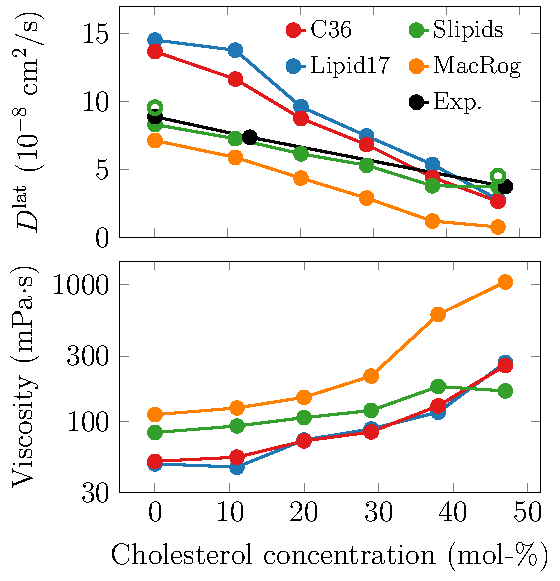
\includegraphics[width=8.7cm]{../FIGS/dynamics.pdf}
  \caption{\label{fig:dynamics}%
  \textbf{Dynamic properties of the POPC/cholesterol mixtures.}
  Top: Lateral diffusion coefficients corrected for finite-size effects using Eq.~\eqref{eq:dpbc}. Experimental data are taken from NMR measurements on well-hydrated samples \cite{filippov2003influence,filippov2003effect}. The hollow circles show data extracted for Slipids using a shorter Lennard-Jones cutoff (see text).
  %
  Bottom: Shear viscosities obtained from the finite-size correction.
  %
  The size-dependence of lateral diffusion and the fits used to obtain the PBC-corrected diffusion coefficients and shear viscosities are shown in Figs.~\ref{SIfig:dvssize} and \ref{SIfig:dvschol}.
  }
\end{figure}

The lipid models again show significantly different behavior. CHARMM36 and Lipid17 provide drastically too large diffusion coefficients at low CHOL concentrations, yet they converge towards experimental estimates. This similar behavior is somewhat surprising, as they behave very differently in terms of both area per POPC (Fig.~\ref{fig:densmaps}) and acyl chain ordering (Fig.~\ref{fig:OPmaps}). For CHARMM36, the excessive ordering observed at high CHOL concentrations counterbalances the too fast dynamics observed at low CHOL concentrations. However, the behavior of Lipid17 cannot be explained by the order parameters, as they agree with experiment across CHOL concentrations. The area per POPC is exaggerated at all CHOL concentrations, yet the deviation from experiment decreases towards larger CHOL concentrations. Thus, it seems that CHARMM36 dynamics correlate with chain ordering, whereas those of Lipid17 go hand in hand with area per POPC. With MacRog, the dynamics of POPC are already slightly too slow compared to experiment, and the excessive ordering at large CHOL concentrations leads to a larger underestimation of the experimental values. Curiously, Slipids provides an essentially quantitative agreement with experiment across the studied CHOL concentrations, and thus significantly outperforms other force fields in terms of lateral dynamics. 

Slipids has the largest Lennard-Jones (LJ) cutoff of the used force fields of 1.4~nm (see Table~\ref{SItab:params}), and this cutoff is known to affect dynamic properties \cite{leonard2018comparison}. Therefore, we repeated simulations at 0~mol-\% and 47~mol-\% CHOL for Slipids but with a cutoff of 0.9~nm corresponding to that of Lipid17, and the PBC-corrected diffusion coefficient values are shown in the top panel of Fig.~\ref{fig:dynamics} as hollow green circles. The decrease in cutoff indeed leads to a minor increase in the lateral diffusion coefficient. However, the LJ cutoff alone does not explain the differences between force fields, indicating that they truly spark from differences in the force field interaction parameters.

As the results in Fig.~\ref{SIfig:dvschol} demonstrate, the PBC correction can qualitatively change the trends observed for diffusion coefficients. This results from the fact that the size of the PBC correction, Eq.~\eqref{eq:sdlatpbc}, depends on membrane viscosity, which further depends on CHOL concentration. For example, Lipid17 and CHARMM36 underestimate the experimental values in all system sizes used here and the effect of CHOL seems to be well reproduced. However, the corrected values significantly overshoot the experiment at low CHOL concentration, and CHOL induces a more drastic slowdown in simulations so that the simulations and experiment almost agree at 47~mol-\% CHOL. With MacRog, even the corrected values fall below the experimental ones, yet the slowdown effect of CHOL is again stronger than in experiment. Slipids is a clear outlier, as the CHOL-dependence seems too weak with finite system sizes, yet after accounting for PBC effects, the agreement with experiment is excellent. These results highlight that little can be said about CHOL-dependence of lateral diffusion coefficients without performing multiple simulations required for the PBC correction at multiple CHOL concentrations. When fine-tuning interaction parameters, this can lead to a massive number of simulations.

The PBC correction, Eq.~\eqref{eq:sdlatpbc} also provides the shear viscosity of the membrane as a fitting parameter. Instead of shear viscosity, the surface viscosity is sometimes reported, yet this is simply the product of shear viscosity and membrane thickness (available in Fig.~\ref{fig:densmaps}). The shear viscosity values are in line with the lateral diffusion coefficients. 

\subsection{Cholesterol Induces Order in a Non-collective Manner}

CHOL could induce order in a lipid membrane in two ways; it could either increase the average order of all phospholipids (``collective transition''), or increase the prevalence of the ordered lipids (``two state model''). To clarify this effect, we extracted the C--H angle distributions with respect to the $xy$ plane for the last six carbons of the palmitate chain from all force fields. We first accumulated data at all CHOL concentrations, and observed that these data could be fitted with two Gaussian functions. These Gaussians were centered at 0$^\circ$, and with the different standard deviations they corresponding to the more and less ordered acyl chains. The obtained standard deviations for the more and less ordered chains only showed minor differences between the force fields (rightmost panel in Fig.~\ref{SIfig:chdist}). We then fitted the C--H angle distributions for all CHOL concentrations with the two Gaussians with the obtained standard deviations and with their means set to 0. These Gaussians provided provided excellent fits to the data with $R^2=0.991\pm 0.005$ (see the leftmost panel of Fig.~\ref{SIfig:chdist} for the fits to the Slipids data). The prefactors of the Gaussian functions were considered to represent the fractions of the more and less ordered components in the system. In pure POPC, the ordered component was absent, yet its prevalence increased linearly as a function of CHOL, after saturating at high CHOL concentrations (rightmost panel in Fig.~\ref{SIfig:chdist}). The success of the two-Gaussian fits in describing the data indicates that with all force fields the bilayer is composed of lipids ordered by CHOL and lipids corresponding to their state in pure POPC membrane, \textit{i.e.} corresponding to the ``two state model'', and CHOL simply changes the fraction of these two states present. Indeed, single Gaussian fits with the standard deviation as a free parameter fail when CHOL is present, indicating that the ordering does not occur \textit{via} a ``collective transition''.

\subsection{Quality of Force Fields at Various Cholesterol Concentrations}

The previous sections highlight that the agreement of the studied force fields with experiment depends on both the parameter in question or the CHOL concentration. To capture these features in an easily digestible form, we have calculated the relative deviations of the density profiles, the order parameters of the two acyl chains, and the diffusion coefficients between the experiments and all the force fields. The interpolated data were used, and the relative deviation from experiments was obtained by dividing the difference of simulated and experimental data by the latter. These data are shown in the two leftmost columns in Fig.~\ref{fig:deviation} as stacked plots.

\begin{figure}[htb!]
  \centering
  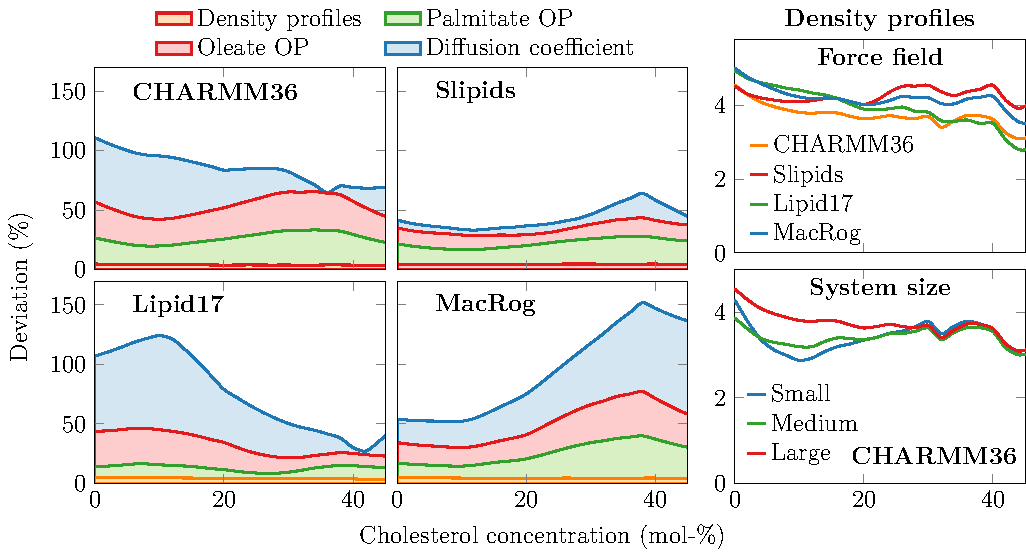
\includegraphics[width=\linewidth]{../FIGS/deviation.pdf}
  \caption{\label{fig:deviation}%
  \textbf{Total deviation of the force fields from experimental data.} 
%
  Two leftmost columns:
  The relative deviations from the first two minima in the form factor), palmitate and oleate chain order parameters, and diffusion coefficients are shown in a cumulative manner to highlight the overall deviation of the force fields from experimental data.
  %
  The order parameter deviations are obtained by averaging over the columns in Fig.~\ref{fig:OPmaps} and normalizing against experimental data. The differences in the form factor minima in Fig.~\ref{fig:SIfig:ffminima} between experiment and simulation were calculated, normalized against experimental data, and summed together. The diffusion coefficient deviation is the difference of values from simulation and experiment in Fig.~\ref{fig:dynamics}, taken after interpolation to the same CHOL values as shown in Figs.~\ref{fig:OPmaps} and \ref{fig:densmaps}, and normalized against experimental values.
%
  Top right panel: 
  The zoomed-in view to the deviation in the location of the first minimum in the form factor.
%
  Bottom right panel:
  Deviation of the density profiles calculated from the form factor using the SDS model. The density profile deviations are calculated as the difference between the simulation and experimental maps in Fig.~\ref{fig:densmaps} followed by averaging over the columns and normalization against experiment.
  }
\end{figure}

\todo{adjust text to highlight changes in Fig.~\ref{fig:deviation}}
\todo{include description of Fig.~\ref{SIfig:ffminima}}

It is evident that the diffusion coefficients and order parameters (``OPs'') contribute more to the total deviation than the density profiles, and the latter are barely visible in the two leftmost columns of Fig.~\ref{fig:deviation}. Therefore, the density profile deviations for the different force fields are shown also in the top right panel of Fig.~\ref{fig:deviation}, which reveals fairly similar deviations of 3--5\% for all force fields. The lower left panel shows the effect of system size on the deviation of CHARMM36 density profiles from experiment. Fig.~\ref{SIfig:densprofssize} demonstrated that smaller systems have more sharp density peaks due to smaller fluctuations, and the small and medium systems indeed agree slightly better with experiment at low CHOL concentrations. However, at larger CHOL concentrations the membranes become stiffer, the smearing caused by the bilayer fluctuations is eliminated, and the deviation from experiment is similar with all system sizes. 

Coming back to the comparison of force fields in the two leftmost columns of Fig.~\ref{fig:deviation}, we see that CHARMM36 and MacRog never provide the best overall agreement with experiment. The latter performs relatively well at low CHOL concentrations, but its quality deteriorates significantly upon the addition of CHOL. At low CHOL concentration, Slipids provides the best agreement with experiment, yet its quality decreases slightly at higher CHOL concentrations. Still, Slipids is the second best force field even in the high CHOL regime. Lipid17 provides the worst agreement with experiment at low CHOL concentrations, but improves significantly towards larger concentrations so that at above $\sim$30~mol-\% of CHOL, Lipid17 provides the best overall agreement with experiment. 

\subsection{Molecular Level Structure of PC--CHOL Mixtures}

Molecular dynamics simulations provide a description of the molecular organization of POPC and CHOL in the bilayer, yet the reliability of this description depends on the quality of the used force field. In the previous section we established that Slipids and Lipid17 provide the best agreement with experimental properties at low and high CHOL concentrations, respectively. Thus, it is reasonable to assume that the molecular pictures provided by these two force fields at the corresponding CHOL concentration regimes are the most realistic.

Eearlier studies have analyzed the organization of CHOL and DSPC chains and observed five and three density peaks for DSPC chains and other CHOL molecules around CHOL molecules \cite{martinez2010cholesterol}. 

\textcolor{red}{2D DENSITY MAPS HERE}

Apart from the lateral organization of the molecules, their orientations might also differ between the force fields. However, we observed only small differences in the tilt of CHOL molecules, defined by the angle between a vector spanning the rigid ring structure as well as the $z$ axis (membrane lies in the $x,y$ plane). The mean angles and their standard deviations are shown in Fig.~\ref{SIfig:choltilt}. Lipid17 and Slipids show very consistent values. CHARMM36 has slightly smaller tilt angles than them across all CHOL concentrations. MacRog has the most tilted CHOL molecules at low CHOL concentrations, but their tilt angle is the smallest at large CHOL concentrations. Still, the differences are overall minor.

\section{Conclusions}

To conclude, the recent all-atom force fields all capture the overall trends of CHOL--PC interaction reasonably well; The addition of CHOL leads to acyl chain ordering, which goes hand in hand with the increase in bilayer thickness. Area per lipid increases less than what would be expected if the areas of POPC and CHOL were additive, manifesting a condensation effect of CHOL. However, beyond these qualitative features, the force fields behave very differently. At the physiological CHOL concentrations in the range from 0 to 30~mol-\%, CHOL has a positive partial area in Slipids and Lipid17, a zero partial area in CHARMM36, and a negative partial area in MacRog. In addition to these trends, the absolute values of area per lipid and bilayer thickness vary substantially. At larger CHOL concentrations all force fields predict a too thick membrane, indicating an excessive ordering effect of CHOL. This is indeed verified by the order parameter maps, which suggest that the palmitate chain is overly ordered in all force fields to a varying degree. The best agreement with experiment is achieved with Slipids at low CHOL concentration and with Lipid17 at high CHOL concentration. In terms of dynamics, the lateral diffusion in pure POPC is too fast in Lipid17 and CHARMM36, and the addition of CHOL slows them both down more than in experiments. MacRog has overall too slow dynamics, whereas Slipids agrees quantitatively with the experiment, indicating that it provides the best description of lipid diffusion.

None of the force fields is clearly the best. Slipids shows great description of lateral dynamics, and reasonable behavior in terms of membrane thickness and acyl chain ordering. Lipid17 provides the best description for the acyl chain ordering, but is otherwise in a relatively poor agreement with experiment. Thus, the choice of force field depends not only on the choice of membrane properties (strutural vs. dynamic) relevant to the problem, but also on the CHOL concentration range of interest. At low  concentrations, Slipids is a safe choice, but at higher concentrations Lipid17 might provide the most realistic description. Since many research questions will involve other lipids, proteins, sugars, or drugs, so the quality of the force fields describing these additional molecules might be the decisive factor, together with force field compatibility. Finally, it must be noted that while all simulations were performed with their suggested simulation parameters, the different simulation engines might provide slightly different behavior, yet we believe that evaluating the magnitude of these effects is well beyond the scope of this work.

\section{Acknowledgements}
We acknowledge CSC -- IT Center for Science for computational resources.
%
JJM thanks the Amber community (Benjamin Madej from the Walker lab and Callum Dickson from the Gould lab) for technical assistance related to the lipid14 force field parameters. 
%
MJ thanks the Academy of Finland (Postdoctoral researcher grant no. 338160) and the Emil Aaltonen foundation for funding.

\bibliography{refs.bib}

%\newpage
%\section{APPENDIX: The NMR results reported by Tiago Ferreira}

\listoftodos

\end{document}

\begin{table*}[]
  \centering
  \caption{Simulated lipid bilayers containing cholesterol. The simulation file data sets marked with $^*$ include also part of the trajectory.
    $^a$ The number of lipid molecules
    $^b$ The number of cholesterol molecules
    $^c$ Cholesterol concentration (mol\%)
    $^d$ The number of water molecules
    $^e$ Simulation temperature
    $^f$ The total simulation time
    $^g$ Time frames used in the analysis
    $^h$ Reference link for the downloadable simulation files
    $^i$ Reference for the full simulation details
  }\label{systemsCHOL}
  \begin{tabular}{c c c c c c c c c c c}
    %\hline
    Force field & lipid   & $^a$N$_{\rm l}$ & $^b$N$_{\rm chol}$ &$^c$C$_{\rm CHOL}$  &  $^d$N$_{\rm w}$ & $^e$T (K)  & $^f$t$_{{\rm sim}}$(ns)  & $^g$t$_{{\rm anal}}$ (ns)& $^h$Files  &  $^i$Details\\
    \hline
    Berger-POPC-07~\cite{ollila07a}&   POPC &128 & 0 &0\% & 7290  & 298  & 270 & 240 & [\citenum{bergerFILESpopc}]$^*$ & [\citenum{ferreira15}] \\
    /H\"oltje-CHOL-13~\cite{holtje01,ferreira13}   &    & &  &   &   &  &  &  &  \\
    &   POPC &120 & 8 & 6\% &7290   & 298  & 100 & 80 & [\citenum{bergerFILESpopc7chol}]$^*$ & [\citenum{ferreira13}] \\
    &   POPC &110 & 18& 14\% & 8481  & 298  & 100 & 80 & [\citenum{bergerFILESpopc15chol}]$^*$ & [\citenum{ferreira13}]  \\
    &   POPC &84 & 44 & 34\%  & 6794   & 298  & 100 & 80 & [\citenum{bergerFILESpopc34chol}]$^*$ & [\citenum{ferreira13}] \\
    &   POPC &64 & 64 & 50\% & 10314  & 298  & 100 & 80 & [\citenum{bergerFILESpopc50chol}]$^*$ & [\citenum{ferreira13}] \\
    &   POPC &50 & 78 & 61\% & 5782   & 298  & 100 & 80 & [\citenum{bergerFILESpopc60chol}]$^*$ & [\citenum{ferreira13}] \\
CHARMM36\cite{klauda10,lim12}  & POPC   & 200& 0& 0\% & 9000  & 310  & ? & 100 & [\citenum{charmm36gromacs5chol0-30}]$^*$  &  SI   \\
                               & POPC   & 200& 22& 10\% & 9000  & 310  & ? & 100 & [\citenum{charmm36gromacs5chol0-30}]$^*$  &  SI   \\
                               & POPC   & 200& 50& 20\% & 9000  & 310  & ? & 100 & [\citenum{charmm36gromacs5chol0-30}]$^*$  &  SI   \\
                               & POPC   & 200& 86& 30\% & 9000  & 310  & ? & 100 & [\citenum{charmm36gromacs5chol0-30}]$^*$  &  SI   \\
                               & POPC   & 200& 134& 40\% & 15030  & 310  & 109 & 100 & [\citenum{charmm36gromacs5chol40-50}]$^*$  &  SI   \\
                               & POPC   & 200& 200& 50\% & 18000  & 310  & 109 & 100 & [\citenum{charmm36gromacs5chol40-50}]$^*$  &  SI   \\
Slipids\cite{jambeck12b,jambeck12,jambeck13b}  & POPC   & 200 & 0 & 0\%   & ?  & 310 & ? & 100 & [\citenum{slipidsCHOL0-30T310}]$^*$ & SI  \\
                                               & POPC   & 512 & 0 & 0\%   & 23943  & 310 & 170 & 100 & [\citenum{slipidsCHOL0T298}]$^*$ & SI  \\
                                               & POPC   & 200 & 22 & 10\% & ?  & 310 & ? & 100 & [\citenum{slipidsCHOL0-30T310}]$^*$ & SI  \\
                                               & POPC   & 200 & 50 & 20\% & ?  & 310 & ? & 100 & [\citenum{slipidsCHOL0-30T310}]$^*$ & SI  \\
                                               & POPC   & 200 & 86 & 30\% & ?  & 310 & ? & 100 & [\citenum{slipidsCHOL0-30T310}]$^*$ & SI  \\
                                               & POPC   & 358 & 154 & 30\% & 21183  & 298 & 170 & 100 & [\citenum{slipidsCHOL30T298}]$^*$ & SI  \\
                                               & POPC   & 200 & 134 & 40\% & ?  & 310 & 109 & 100 & [\citenum{slipidsCHOL40-50T310}]$^*$ & SI  \\
                                               & POPC   & 200 & 200 & 50\% & ?  & 310 & 109 & 100 & [\citenum{slipidsCHOL40-50T310}]$^*$ & SI  \\
                                               & POPC   & 256 & 256 & 50\% & 20334  & 298 & 170 & 100 & [\citenum{slipidsCHOL50T298}]$^*$ & SI  \\ 
     MacRog\cite{kulig15b}     & POPC   & 128 & 0 & 0\% & 6400  & 310 & 400 & 200 & [\citenum{macrogCHOLfiles}]$^*$ & [\citenum{botan15}] \\ 
                          & POPC   & 114  & 14 & 11\% & 6400  & 310  & 400 & 200 & [\citenum{macrogCHOLfiles}]$^*$ & [\citenum{botan15}]    \\
                          & POPC   & 72   & 56 &  44\% & 6400  & 310  & 400 & 200 & [\citenum{macrogCHOLfiles}]$^*$ & [\citenum{botan15}]    \\
                             & POPC   & 64  & 64 & 50\% & 6400  & 310  & 400 & 200 & [\citenum{macrogCHOLfiles}]$^*$ & [\citenum{botan15}]    \\
                             & POPC   & 56   & 72 & 56\% & 6400  & 310  & 400 & 200 & [\citenum{macrogCHOLfiles}]$^*$ & [\citenum{botan15}]    \\
     Lipid14\cite{walker14,walker15}     & POPC   & 120 & 8 & 6\% &  3968 & 303 & 200 & 200 & [\citenum{lipid14sys1}]$^*$ & SI \\ 
                          & POPC   & 108  & 20  & 16\% & 3968  & 303  & 200 & 200 & [\citenum{lipid14sys2}]$^*$ & SI    \\
                          & POPC   &  84  & 44 &  34\% & 3968  & 303  & 200 & 200 & [\citenum{lipid14sys3}]$^*$ & SI    \\
                             & POPC   & 64  & 64 & 50\% & 3968  & 303  & 200 & 200 & [\citenum{lipid14sys4}]$^*$ & SI    \\
                             & POPC   &  52  & 76 & 59\% & 3968  & 303  & 200 & 200 & [\citenum{lipid14sys5}]$^*$ & SI    \\
\end{tabular}
\end{table*} 



\begin{figure}[]
 \centering
 \includegraphics[width=8cm]{../FIGS/FormFactors.eps}
 \caption{\label{FormFactors}
   Form factors from simulations and experiments.
 }
 \todo{Details about form factor calculation code is discussed in issues
   https://github.com/NMRLipids/MATCH/issues/56 and https://github.com/NMRLipids/MATCH/issues/50.
   Once the code is finalized, we should recalculate and check the form factors.
   CURRENTLY, 10\%-40\% cholesterol concetrations are calculated with a code which gives possibly incorrect
   heigths for the maxima.
 } \\
 \todo{The y-axis scale cannot be explicitly measured in experiments.
   Therefore, the y-axis of the experimental form factor is typically scaled to match with simulations.
   This currently not done, because we have several simulations which give inequal form factors, and therefore
   it is not clear against which simulation results we should scale the experimental results.
   I have created a issue for this discussion: https://github.com/NMRLipids/NmrLipidsCholXray/issues/18
 } \\
 \todo{Not all experimental and simulation data is here (maybe?).}
\end{figure}
\begin{figure}[]
  \centering
  \includegraphics[width=8cm]{../FIGS/apls.eps}
  \caption{\label{apls}
    Area per molecules calculated from different simulation models
    as a function of cholesterol concentration. The solid symbols are area per
    total amount of molecules (chol+PC) and the empty symbols area per PC headgroups.
    Top figure shows absolute values and bottom figure shows changes respect
    to pure lipid system.
  }
\end{figure}



Visual inspection of form factors (Fig. \ref{FormFactors}) and quantitative quality estimation (Fig. \ref{FormFactorsFITNESS})
suggests that the Berge/Holtje force field gives the best agreement with experiments with large
cholesterol concentration. This is surprising because the same model overestimated acyl chain
order parameter increase upon addition of cholesterol more than CHARMM36 or Slipids simulations
(Figs. \ref{OrderParametersCHOL} and \ref{OrderParametersCHOLchanges}).
The Berger/Holtje model also exhibits the most pronounced decrease in the area per molecule
upon addition of cholesterol (Fig. \ref{alps}).
On the other hand, the electron density profiles from Berger/Holtje simulations are closer
to the result from the SDP model then other MD simulation models for both pure POPC bilayer
and equimolar POPC/cholesterol mixture, especially in the middle of the bilayer
where SDP model gives substantially lower density than MD simulations (Fig. \ref{densities}).
Therefore, the good quality of form factor Berger/Holtje model with large amounts of cholesterol
may rather indicate the importance of this low electron density in the bilayer center,
rather than better quality of lipid-cholesterol interactions in this model.
\begin{figure}[]
  \centering
  \includegraphics[width=8cm]{../FIGS/FFfitness.eps}
  \caption{\label{FormFactorsFITNESS}
    Fitness of form factors between simulations and experiments.
  }
    \todo{Figure to be done properly when the fitness code is finished.
    This is discussed in issues
    https://github.com/NMRLipids/MATCH/issues/65,
    https://github.com/NMRLipids/MATCH/issues/64,
    https://github.com/NMRLipids/MATCH/issues/56, and
    https://github.com/NMRLipids/MATCH/issues/50
  }
\end{figure}

The overestimation of order parameters observed in CHARMM without cholesterol and in all force fields
with cholesterol is smaller than the contribution by undulations in large simulations (section \ref{undulations} in the supplementary information).
\begin{figure}[]
  \centering
  \includegraphics[width=8cm]{../FIGS/slopes.eps}
  \caption{\label{OrderParametersCHOLchanges}
    Slopes of order parameters as a function of cholesterol.
    Determined by fitting equation $S_{\rm CH}(C_{\rm chol})=k_{\rm OP}C_{\rm chol}+S_{\rm CH}(0)$
    to the data in figures \ref{slopes}-\ref{slopesslipids310K}.
  }
  \todo{It would be good to plot these slopes from also other experimental data in the literature.}
\end{figure}

% \begin{figure}[]
%   \centering
%   \includegraphics[width=8cm]{../FIGS/densitiesEXTREMES.eps}
%   \caption{\label{densities}
%     Electron density profiles from MD simulations and SDP model.
%   }
% \end{figure}

\begin{figure*}[]
  \centering
  \includegraphics[width=17.2cm]{../FIGS/OrderParametersCHOLfitness.eps}
  \caption{\label{OrderParametersCHOLfitness}
    Difference between order parameters from simulations and experiments for acyl chains of  1-palmitoyl-2-oleoylphosphatidylcholine (POPC).
  }
  \todo{Figure to be done properly when the fitness code is finished.
    This is discussed in issues
    https://github.com/NMRLipids/MATCH/issues/65,
    https://github.com/NMRLipids/MATCH/issues/64,
    https://github.com/NMRLipids/MATCH/issues/56, and
    https://github.com/NMRLipids/MATCH/issues/50
  }
\end{figure*}

% \begin{figure*}[]
%   \centering
%   \includegraphics[width=17.2cm]{../FIGS/OrderParametersCHOL.eps}
%   \caption{\label{OrderParametersCHOL}
%     Order parameters from simulations and experiments for acyl chains of  1-palmitoyl-2-oleoylphosphatidylcholine (POPC).
%   }
%   \todo{Lipid14 results?} 
% \end{figure*}


\subsection{Presenting the quality of lipid bilayer MD simulation with binary mixtures}  

All the tested MD simulation models qualitatively reproduced experimentally observed condenced and
ordering effects of cholesterol. However, the acyl chain ordering was overestimated and quality
of form factors reduced with increasing amount of cholesterol. Although the biological importance
of these details is unclear, overestimated ordering may promote formation of liquid ordered phases and
inaccuate form factors complicate interpretation of scattering experiment with MD simulations.
Therefore, MD simulation force fields correctly reproducing the order effects upon addition of the
cholesterol would be invaluable.

To facilitate the comparison of the quality of complex lipid bilayers,
we introduce the quantitative quality measures which measure the quality of
intermolecular interactions in binary lipid bilayers from different perspectives.
The simple difference between experimental and simulated C-H bond order parameters
give a very detailed picture about the quality of molecular conformations in all
positions of lipid bilayer (Fig. \ref{OrderParametersCHOLfitness}).
However, complexity of such presentation increases with increasing amount of data
and it may be hard to present in practical format readable for human or machine.
Using root mean square deviation across regions in the molecule simplifies the presentation,
but compromizes the spatial resolution. Here, we divide the lipid into headgroup, glycerol
backbone, sn-1 and sn-2 chains to present quality of binary lipid bilayer in more convenient
format (Fig. \ref{OrderParametersCHOLfitness}).
\todo{Discussion to be finished once we have the fitness function defined.}